\documentclass[aps, prb, twocolumn, a4paper, floatfix, reprint]{revtex4-2}
\usepackage[%
    margin=10mm,% ако не си принтира 10мм не изглежда грозно, а може да събереш повече текст
    % showframe=true,%
    ]{geometry}
\usepackage[T1,T2A]{fontenc}
\usepackage[utf8]{inputenc}
\usepackage[main=bulgarian, english]{babel}
\usepackage{float}
\AtBeginDocument{\selectlanguage{bulgarian}}
\newcommand{\degree}{^{\circ}}
\usepackage{amsmath}
\usepackage{graphics}
\usepackage{graphicx}
\graphicspath{{.}}
\newcommand{\abs}[1]{\lvert#1\rvert}
\let\phi\varphi
\usepackage{booktabs} % от тук се използва само \midrule може и без него 
%\usepackage{adjustbox} % това може да се използва, за да „смаляваш“ широки таблици
%\usepackage{tabularx} % дефинира колона X в среда tabularx която добавя празно място така че цялата таблица да запълни определена ширина
\usepackage{dcolumn}
\newcolumntype{d}[1]{D{.}{.}{#1}}
\usepackage[unicode=true,pdfusetitle]{hyperref}


\makeatletter
\renewcommand{\Dated@name}{}%
\makeatother



\begin{document}
\title{Еластично усукване}
\author{Васил Николов}
\noaffiliation
\date{21.11.2021}
\maketitle

\section{Цел на упражнението}
Да се измери модулът на срязване $G$ на алуминия и да се провери линейната зависимост на ъгълът на усукване на тънка метална пръчка от приложеният й въртящ момент.

\section{Експериментална установка}
Единият край на тънка метална пръчка е застопорен, а на другият е закрепена макара, чрез която на пръчката може да се прилага въртящ момент. На макарата има скала, която може да измерва ъгълът на усукване на пръчката $\phi$. От двете страни на макарата са закачени нишки, които са прехвърлени през две други макари, и на които може да се закачат тежести. Така с различни тежести на пръчката се прилага различен въртящ момент.

\section{Теоретична обосновка}
Теоретично може да се изведе, че ъгълът на усукване зависи по следният начин от параметрите на системата:
\begin{equation*}
    \phi=\frac{Tl}{JG}
\end{equation*}
където $T$ е приложеният въртящ момент, $l$ е дължината на пръчката, $J$ е площният инерционен момент, $G$ е модулът на срязване на алуминия. Знаейки параметрите на системата можем да определим напълно всички тези променливи освен $G$

\begin{gather*}
    T=2mgR \\
    J=\pi/2 r^4 \\
    \phi = \frac{4LRmg}{\pi r^4 G} \label{eq:1} \tag{1}
\end{gather*}
От горното уравнение се вижда, че зависимостта на ъгълът от окачената маса е линейна. На графика
\begin{gather*}
    y=\phi , \ \ x=m \\
    \frac{dy}{dx} = \frac{4LRg}{\pi r^4 G} \\
    G = \frac{4LRg}{\pi r^4 \frac{dy}{dx}} \label{eq:2} \tag{2} 
\end{gather*}

\section{Експериментални данни и резултати}

\begin{figure}[H]
    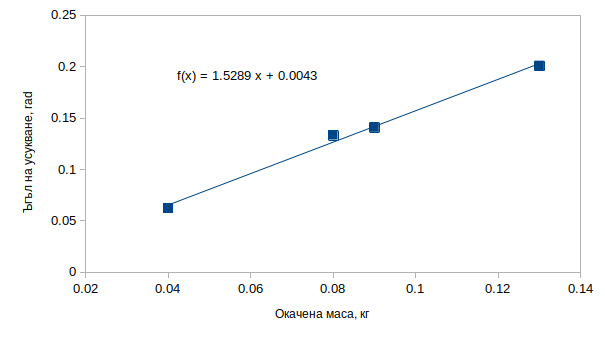
\includegraphics[width=0.9\columnwidth, keepaspectratio=true]{angle_vs_mass_chart.png}
\end{figure}

От графиката на ъгълът на усукване като функция на окачената маса можем да измерим $\frac{dy}{dx} = 1.53 \ kg^{-1}$, и по \eqref{eq:2} 
\begin{equation}
    G = 28.4 \ GPa \pm 5\%
\end{equation}
Тази стойност е близка до табличната стойност за алуминия. 

\end{document}